%% Additional propositional calculi retained after exact source restoration.
\noindent\textit{Reader note.} The following Hilbert, tableau, and
comparison material is a separately attributed addition to the inherited
chapter above; it neither alters nor replaces the exact source rule displays.

The retained Hilbert presentation and deduction theorem are attributed to
\cite{Mendelson1997}.

\section{Hilbert calculus and the deduction theorem}
\label{sec:p02-hilbert-cpl}

\begin{hbdefinition}{def:p02-hilbert-derivation}{Classical propositional Hilbert derivation}
Let \(\mathsf H_{\mathsf{CPL}}\) be the calculus in registry sheet
\hyperref[sheet:hilbert-cpl]{\texttt{sheet:hilbert-cpl}}.  Its language is the
\(\{\neg,\to\}\)-fragment.  For a set \(\Gamma\) of formulas in that
fragment, a \emph{Hilbert derivation from \(\Gamma\)} is a finite sequence
whose every member is in \(\Gamma\), is a uniform-substitution instance of
one of the three axiom schemas on the sheet, or follows from two earlier
members by the sheet's sole inference rule.  Write
\(\Gamma\derives_{\mathsf H_{\mathsf{CPL}}}\theta\) exactly when such a
sequence ends in \(\theta\).  This sequential notion is distinct from the
discharge-labelled trees above; the next theorem supplies the controlled
way to internalize one premise.
\end{hbdefinition}

\begin{hbtheorem}{thm:p02-hilbert-deduction}{proved=annex:p2.calc.2}{Deduction theorem for the Hilbert calculus}
For every set \(\Gamma\) and all formulas \(\varphi,\psi\) of the
\(\{\neg,\to\}\)-fragment,
\[
 \Gamma\cup\{\varphi\}\derives_{\mathsf H_{\mathsf{CPL}}}\psi
 \quad\Longleftrightarrow\quad
 \Gamma\derives_{\mathsf H_{\mathsf{CPL}}}(\varphi\to\psi).
\]
\end{hbtheorem}

\begin{hbdefinition}{def:p02-hilbert-translation}{Full-language-to-Hilbert translation}
The Hilbert sheet uses only \(\neg,\to\), whereas the other calculi use the
full primitive language, so a grammar-changing map is necessary before their
derivability relations can be compared without ambiguity.  Fix the
propositional variable \(p_0\).  Define the metalinguistic recursive map
\(\operatorname{tr}_{\mathsf H}:\mathsf{Fm}_{\mathsf{CPL}}\to
\mathsf{Fm}_{\{\neg,\to\}}\) by
\[
\begin{aligned}
 \operatorname{tr}_{\mathsf H}(p)&\defeq p,
 &\operatorname{tr}_{\mathsf H}(\bottom)&\defeq\neg(p_0\to p_0),
 \\
 \operatorname{tr}_{\mathsf H}(\neg\alpha)&\defeq
   \neg\operatorname{tr}_{\mathsf H}(\alpha),
 &\operatorname{tr}_{\mathsf H}(\alpha\to\beta)&\defeq
   \operatorname{tr}_{\mathsf H}(\alpha)\to
   \operatorname{tr}_{\mathsf H}(\beta),
 \\
 \operatorname{tr}_{\mathsf H}(\alpha\land\beta)&\defeq
   \neg(\operatorname{tr}_{\mathsf H}(\alpha)\to
        \neg\operatorname{tr}_{\mathsf H}(\beta)),
 \\
 \operatorname{tr}_{\mathsf H}(\alpha\lor\beta)&\defeq
   \neg\operatorname{tr}_{\mathsf H}(\alpha)\to
        \operatorname{tr}_{\mathsf H}(\beta).
\end{aligned}
\]
Here \(p\) ranges over propositional variables and
\(\operatorname{tr}_{\mathsf H}[\Gamma]\defeq
\{\operatorname{tr}_{\mathsf H}(\gamma):\gamma\in\Gamma\}\).  The map is not a
new connective and not the formula-equivalence relation \(\Leftrightarrow\):
it changes the grammar while preserving each formula's classical truth
function.  Its use is the final clause of the next theorem.
\end{hbdefinition}

\begin{hbtheorem}{thm:p02-calculi-derivability-equivalence}{proved=annex:p02-w02b-p02-010-calculi-equivalence}{Derivability equivalence of the classical calculi}
Let \(\Gamma\) be a finite set of full-language propositional formulas and
let \(\varphi\) be a full-language formula.  View \(\Gamma\) as a multiset
with multiplicity one when it forms a sequent antecedent.  Then
\[
\begin{aligned}
 \Gamma\entails\varphi
 &\quad\Longleftrightarrow\quad
 \Gamma\derives_{\mathsf{ND}_{\mathsf{CPL}}}\varphi\\
 &\quad\Longleftrightarrow\quad
 \text{the sequent }\Gamma\Rightarrow\varphi
   \text{ is derivable in }\mathsf{LK}_{\mathsf{CPL}}\\
 &\quad\Longleftrightarrow\quad
 \operatorname{tr}_{\mathsf H}[\Gamma]
   \derives_{\mathsf H_{\mathsf{CPL}}}
   \operatorname{tr}_{\mathsf H}(\varphi).
\end{aligned}
\]
The natural-deduction and sequent presentations are due to Gentzen; see
\cite{Gentzen1934a}.  The Hilbert legs are
\cref{thm:p02-w02b-p02-010-hilbert-equivalence}, obtained from the explicit
derivation maps of \cref{sec:p02-w02b-p02-010-translations}; Gentzen's own
equivalence proof for his calculi is \cite[Abschnitt~V, \S 6, p.~429]{Gentzen1935b}.
\end{hbtheorem}

\begin{hbwarning}{def:p02-derivability-not-proof-identity}{Derivability equivalence is not proof identity}
The preceding theorem compares existence of derivations.  It asserts neither
literal identity of derivation objects nor preservation of proof size, and it
does not assert that an arbitrary translation of a natural-deduction or
Hilbert derivation lands directly in cut-free \(\mathsf{LK}\).  Cut
elimination and its proof transformations are separate Part~7 results.
\end{hbwarning}

\begin{figure}[htbp]
\centering
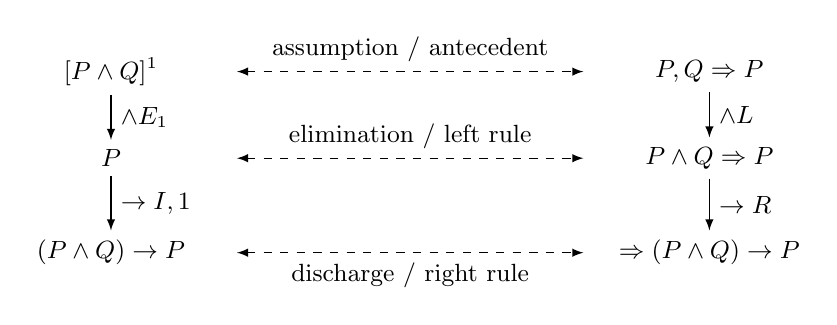
\begin{tikzpicture}[font=\small,>=latex]
  \node (nda) at (-3.8,2.3) {$[P\land Q]^1$};
  \node (ndp) at (-3.8,1.2) {$P$};
  \node (ndi) at (-3.8,0) {$(P\land Q)\to P$};
  \draw[->] (nda) -- node[right] {$\land E_1$} (ndp);
  \draw[->] (ndp) -- node[right] {$\to I,1$} (ndi);

  \node (lki) at (3.8,2.3) {$P,Q\Rightarrow P$};
  \node (lka) at (3.8,1.2) {$P\land Q\Rightarrow P$};
  \node (lkr) at (3.8,0) {$\Rightarrow(P\land Q)\to P$};
  \draw[->] (lki) -- node[right] {$\land L$} (lka);
  \draw[->] (lka) -- node[right] {$\to R$} (lkr);

  \draw[<->,dashed] (-2.2,2.3) -- node[above] {assumption / antecedent} (2.2,2.3);
  \draw[<->,dashed] (-2.2,1.2) -- node[above] {elimination / left rule} (2.2,1.2);
  \draw[<->,dashed] (-2.2,0) -- node[below] {discharge / right rule} (2.2,0);
\end{tikzpicture}
\caption{One natural-deduction/\(\mathsf{LK}\) correspondence.
The arrows exhibit this example's matching steps; they do not claim a
step-for-step equivalence for arbitrary proofs.}
\label{fig:p02-nd-lk-correspondence}
\end{figure}

\section{Analytic tableaux}
\label{sec:p02-analytic-tableaux}

\begin{hbdefinition}{def:p02-cpl-tableau}{Tableau}
For finite \(\Gamma\subseteq\mathsf{Fm}_{\mathsf{CPL}}\), a
\emph{tableau rooted at \(\Gamma\)} is a finite tree of retained branch
lists.  They are built under registry sheet
\hyperref[sheet:tableaux-cpl]{\texttt{sheet:tableaux-cpl}}.  Applying an
expansion appends formulas and marks the principal occurrence as expanded;
it never consumes that occurrence.  A branch is \emph{closed} when it
contains \(\bottom\) or contains both \(\alpha\) and \(\neg\alpha\), and
\emph{open} otherwise.  It is \emph{saturated} when every expandable
occurrence on it is marked.  These marks are metalinguistic bookkeeping, not
formula symbols.  A tableau is closed exactly when every branch is closed.

The root branch lists each member of \(\Gamma\) once; consequence and
validity are tested by rooting at \(\Gamma\cup\{\neg\varphi\}\) and at
\(\{\neg\varphi\}\).  The expandable formulas, expansion steps and finished
tableaux are fixed in
\cref{def:p02-w02-p02-014-input,def:p02-w02-p02-014-expandable}.
\end{hbdefinition}

\begin{hbtheorem}{thm:p02-tableau-adequacy}{proved=annex:p02-w02-p02-014-tableau-adequacy}{Tableau adequacy}
Let \(\Gamma\) be a finite set of propositional formulas.  Every closed
tableau rooted at \(\Gamma\) certifies that \(\Gamma\) is unsatisfiable.
Exhaustively expanding unmarked expandable occurrences
(\cref{def:p02-w02-p02-014-expandable}) terminates in a finite finished
tableau, each of whose branches is closed or saturated.  From any open saturated branch \(B\), define a valuation
by assigning a propositional variable \(p\) true exactly when \(p\) occurs
on \(B\) (and false otherwise).  This branch valuation satisfies every
formula on \(B\), hence every member of \(\Gamma\).  Consequently an
exhaustively expanded saturated tableau has an open branch
exactly when \(\Gamma\) is satisfiable, and it is closed exactly when
\(\Gamma\) is unsatisfiable.
\end{hbtheorem}

\begin{figure}[htbp]
\centering
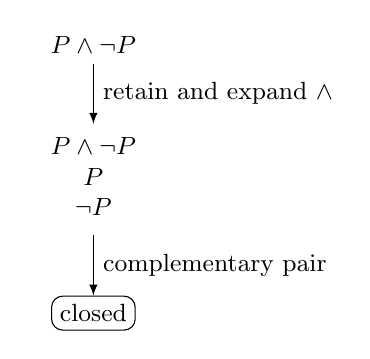
\begin{tikzpicture}[font=\small,>=latex]
  \node (root) at (0,2.7) {$P\land\neg P$};
  \node (expanded) at (0,1.0)
    {$\begin{array}{c}P\land\neg P\\ P\\ \neg P\end{array}$};
  \node[draw,rounded corners,inner sep=3pt] (closed) at (0,-0.7) {closed};
  \draw[->] (root) -- node[right] {retain and expand \(\land\)} (expanded);
  \draw[->] (expanded) -- node[right] {complementary pair} (closed);
\end{tikzpicture}
\caption{A closed propositional tableau for
\(\{P\land\neg P\}\).  The root formula remains on the branch
after expansion; the last node records closure rather than replacing any
formula.}
\label{fig:p02-closed-tableau}
\end{figure}

\begin{landscape}
\section{Proof-system comparison}
\label{sec:p02-proof-system-comparison}

\begingroup\scriptsize\setlength{\tabcolsep}{3pt}
\begin{longtable}{@{}p{.72in}p{1.20in}p{1.80in}p{1.45in}p{1.70in}@{}}
\caption{Classical propositional proof systems side by side.}
\label{tab:p02-proof-systems}\\
\toprule
System & Registry home & Derivation object and rule families & Adequacy form & Proof-search behavior \\ \midrule
\endfirsthead
\caption[]{Classical propositional proof systems side by side (continued)}\\
\toprule
System & Registry home & Derivation object and rule families & Adequacy form & Proof-search behavior \\ \midrule
\endhead
\midrule\multicolumn{5}{r}{\emph{continued on next page}}\\
\endfoot
\endlastfoot
Hilbert & \hyperref[sheet:hilbert-cpl]{\texttt{sheet:hilbert-cpl}} & Finite formula sequence; axiom schemas and one inference rule & Sound and complete after the displayed translation, Theorem~\ref{thm:p02-calculi-derivability-equivalence} & Compact for metatheory; little goal-directed structure \\
Natural deduction & \hyperref[sheet:nd-cpl]{\texttt{sheet:nd-cpl}} & Rooted formula tree; introduction, elimination, and nonvacuous discharge & Sound and complete, same theorem & Goal-directed introductions; eliminations may create detours \\
\(\mathsf{LK}\) & \hyperref[sheet:lk]{\texttt{sheet:lk}} & Tree of finite-multiset sequents; initial, structural, logical, and Cut inferences & Sound and complete, same theorem & Backward search becomes analytic when Cut is excluded; normalization is Part~7 \\
Tableau & \hyperref[sheet:tableaux-cpl]{\texttt{sheet:tableaux-cpl}} & Retained branch lists with linear and splitting expansions & Exhaustive saturated tableau closed iff unsatisfiable; open branch yields a model & Direct refutation search with branch closure and countermodel extraction \\
Resolution & \hyperref[sheet:resolution-cpl]{\texttt{sheet:resolution-cpl}} & Clause sequence generated from inputs by binary resolution & Sound by the inline theorem in \cref{sec:prop-metatheory-04}; finite refutational completeness is \cref{thm:prop-resolution-complete}, with the arbitrary-set extension stated in \cref{rem:resolution-finiteness} & Saturation/search depends strongly on clause choice and redundancy control \\
\bottomrule
\end{longtable}
\endgroup
\end{landscape}
